% !TEX program = pdflatex -> bibtex -> pdflatex*2
\documentclass[twocolumn]{article}
    \usepackage{cite}
    \usepackage{flushend,cuted}
    \usepackage{subfigure}
    \usepackage[pdftex]{graphicx}
    %\usepackage{amsmath,amssymb,amsfonts}
    \usepackage{caption}

% 修改论文题目
% Industrial Robot期刊要求文件不能有作者信息,所以这里只需要准备论文题目即可
\title{Development and Implementation of a Mobile Robot for Road Crack Detection}

% 正文部分
%%%%%%%%%%%%%%%%%%%%%%%%%%% 正文将包含六个部分 %%%%%%%%%%%%%%%%%%%%%%%%%%%%
% abstract                                                              %
% 1. Introduction                                                       %
% 2. Design Goals/Related work                                          %
% 3. Robot Design Specifications                                        %
% 4. Planning and navigation                                            %
% 5. Image Processing                                                   %
% 6. Testing and Experimental Results                                   %
%%%%%%%%%%%%%%%%%%%%%%%%%%% 正文将包含六个部分 %%%%%%%%%%%%%%%%%%%%%%%%%%%%

\begin{document}
\maketitle
%%%%%%%%%%%%%%%%%%%%%%%%%%%%%%%%% 摘要 %%%%%%%%%%%%%%%%%%%%%%%%%%%%%%%%%%%
%%% 摘要:(最多250字)                                                   %
%       1. Purpose(目的)------------------------------------- 必需     %
%       2. Design/methodology/approach(方法)----------------- 必需     %
%       3. Findings(发现)------------------------------------ 必需     %
%       4. Research limitations/implications(限制/启示)------ 非必需    %
%       5. Practical implications(现实意义)------------------ 非必需    %
%       6. Social implications(社会影响)--------------------- 非必需    %
%       7. Originality/value(创意/价值)---------------------- 必需      %
%%%%%%%%%%%%%%%%%%%%%%%%%%%%%%%%% 摘要 %%%%%%%%%%%%%%%%%%%%%%%%%%%%%%%%%%%
    \begin{strip}
        Abstract\\
        Prupose - Please type your text here.\\
        Design/methodology/approach - Please type your text here.\\
        Findings - Please type your text here.\\
        Research limitations/implications - Please type your text here.\\
        Practical implications - Please type your text here.\\
        Social implications - Please type your text here.\\
        Originality/value - Please type your text here.\\
    \end{strip}
       
    \section{Image Processing}
        We hypothesize the crack areas are darkness long continuous areas in the image. The proposed road crack detection algorithm, depicted in Figure \ref{Flowchart of image processing}, 
        comprises four main steps combining Pre-processing, Dynamic thresholding, Morphological operations, and post-processing.\\  

        \begin{figure}[h]
            \centering
            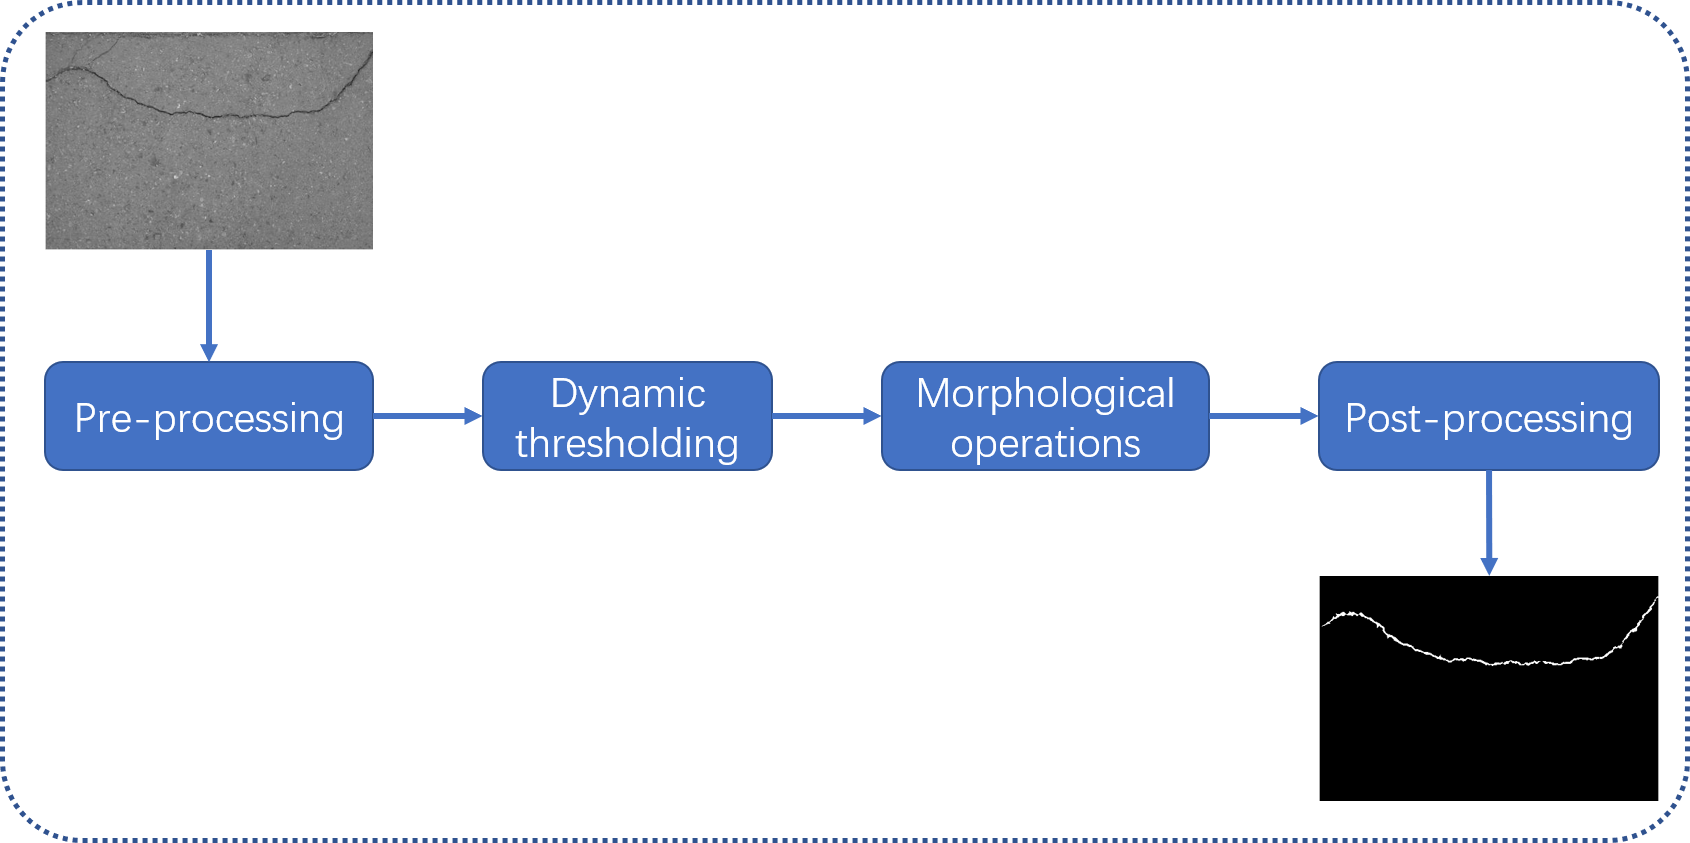
\includegraphics[width=7.5cm]{image//Flowchart_image.png}\\
            \caption{Flowchart of image processing}\label{Flowchart of image processing}
            \end{figure}
        
        \subsection{Pre-processing}
        The pre-processing is adopted to solve the uneven illumination phenomenon. The detailed procudures are:\\
        (1)Estimating the grayscale of the image background. The original image is blocked to calculate the pixel grayscale mean $\mu$ and standard deviation $\sigma$ of this block.
        Then $ max(min,\mu - 3\sigma) $ is taken as the background grayscale of the block, where $min$ is the minimum grayscale value of pixels in the block.\\
        (2)The roughly estimated background grayscale matrix is extended to a matrix of the same size as the original image, thus obtaining the background grayscale matrix.\\
        (3)The original image is subtracted from the background grayscale matrix calculated in the first two steps to correct the uneven illumination.\\
        (4)Top hat transform and bottom hat transform are carried out on the corrected image.The contrast is enhanced by the difference between the top hat transform and the bottom hat transform.\\
        (5)By adjusting the grayscale of the image, the image overdarkening phenomenon caused by subtraction is corrected.\\
        
        \subsection{Dynamic thresholding}
        The Dynamic thresholding is adopted to obtain candidate crack pixels. The neighborhood average value of slide window is taken as local threshold. 
        When the pixel grayscale is less than the local threshold, it is considered to be the suspicious point of crack.\\

        \subsection{Morphological operations}
        After first two steps, some crack area is fractured. Repeating morphological bridging of the processed image to connect fractured crack area, until the image no longer changes. 
        Then morphological close operation is adopted to smooth crack area.\\

        \subsection{Post-processing}
        This step of the proposed method is to keep the longest area in the processed image. According to calculating the length of each connected domain, the connected domain which length is less than 
        the threshold will be removed. Then the final result is obtained.\\ 

    \section{Testing and Experimental Results}  
        \subsection{image processing}
        We capture 118 images from common roads, and we label the groundtruth manually. The example result of proposed algorithm is shown on Figure \ref{Result of image processing}
        In order to evaluate the proposed algorithm ability, there four performance indicators are adopted which are shown in Table \ref{performance}, 
        include accuracy $Acc$, Precision $Pre$, Recall $Re$, Comprehensive evaluation index $F1$, defined as
        $$Acc=\frac{TP+TN}{TP+TN+FP+FN}, Pre=\frac{TP}{TP+FP},$$
        $$Re=\frac{TP}{TP+FN}, F1=\frac{2\times Pre\times Re}{Pre+Re}$$
        where TP, TN, FP, FN are respectively true positive, true negative, false positive, and false negative decisions.\\

        \begin{figure}[h]
            \centering
            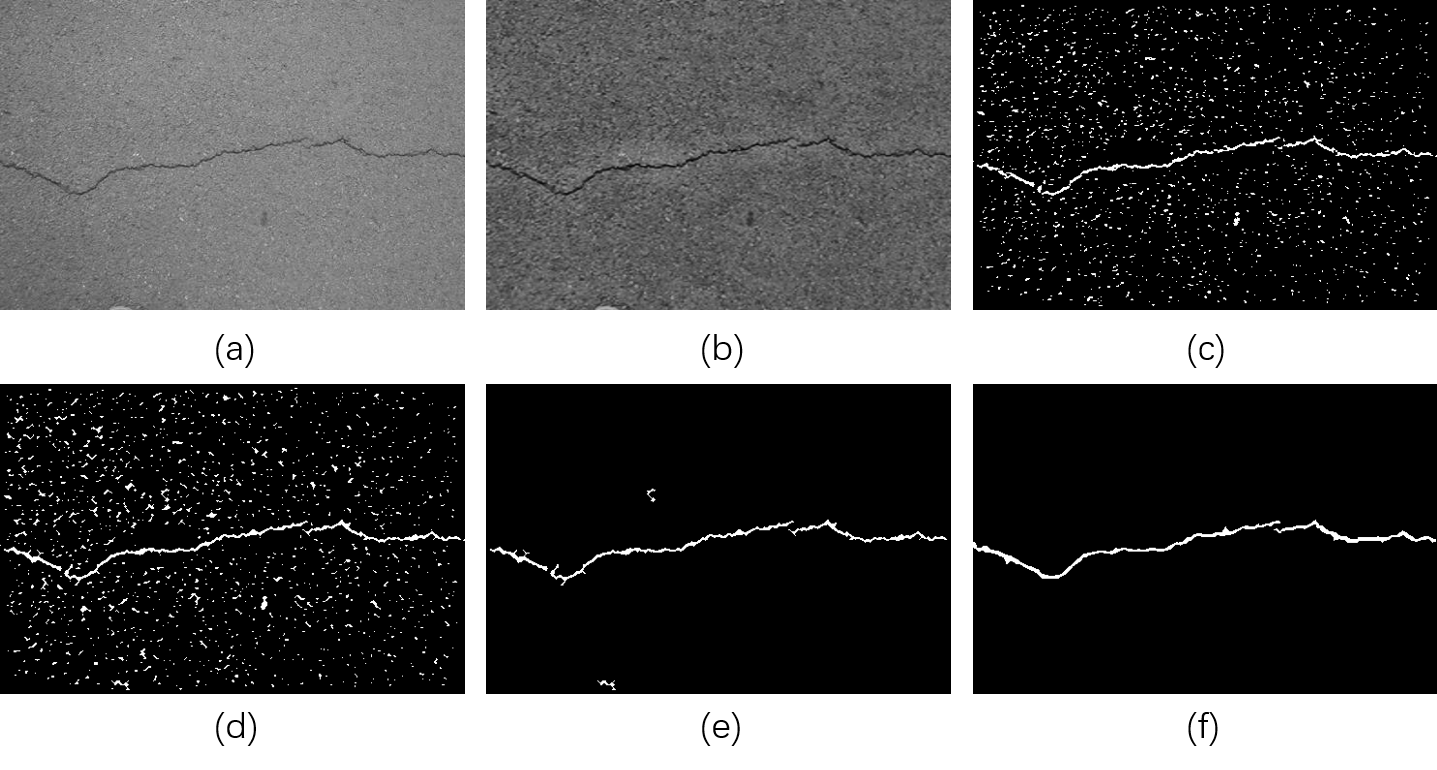
\includegraphics[width=7.5cm]{image//Result_image.png}\\
            \caption{The example result of image processing: (a)Original image; (b)Pre-processing; (c)Dynamic thresholding; (d)Morphological operations; (e)Post-processing; (f)Ground truth.}\label{Result of image processing}
            \end{figure}
        
        \begin{table}[h]
            \centering
            \begin{tabular}{ccccc}
            \hline
            &Acc&Pre&Re&F1\\
            \hline
            result&0.9861&0.5920&0.5026&0.5217\\
            \hline
            \end{tabular}
            \caption{Performance of the proposed method}
            \label{performance}
            \end{table}
            
    \bibliography{info}
    \bibliographystyle{plainnat}
\end{document}
